\documentclass[12pt]{book}
\usepackage[margin=.85in]{geometry} % for MARGIN
\usepackage[many]{tcolorbox}    	% for COLORED BOXES (tikz and xcolor included)


\usepackage{multicol}   
\usepackage{enumerate}
\usepackage[shortlabels]{enumitem}
\usepackage{varwidth}
\usepackage{tasks}
\usepackage[export]{adjustbox}

\usepackage{titleps}
\usepackage{setspace}               % for LINE SPACING
\usepackage[⟨options⟩]{fancyhdr}
\usepackage{enumitem}
\setlist{nosep}
\usepackage{tikz}
\usepackage{pgfplots}
\pgfplotsset{compat=1.5.1}
\usetikzlibrary{datavisualization}
\usetikzlibrary{datavisualization.formats.functions}

\newcommand{\D}{\displaystyle}


\setlength\parindent{0pt}   % killing indentation for all the text
\setstretch{1.3}            % setting line spacing to 1.3
\setlength\columnsep{0.25in} % setting length of column separator
\pagestyle{fancy}           % setting pagestyle to be headings

\usepackage[]{titlesec}

\fancyhead[L]{Math V04 - College Algebra}
\fancyhead[R]{Christina Papazacharioudakis}

\tcbset{
    sharp corners,
    colback = white,
    before skip = 0.2cm,    % add extra space before the box
    after skip = 0.5cm      % add extra space after the box
}                           % setting global options for tcolorbox

    \newtcolorbox{boxR}{
    fontupper = \color{black}, % font color
    boxrule = 1.5pt,
    colframe = black,
    rounded corners,
    arc = 5pt   % corners roundness
}

\definecolor{ballblue}{rgb}{0.13, 0.67, 0.8}

\begin{document}



\begin{comment}
Name: \underline{\hspace{100mm}}
\vspace{20mm}
  \centerline{\Large \textbf{Chapter 2: Equations and Inequalities} } 

{\large
\begin{center}
\begin{varwidth}{\textwidth}
\begin{enumerate}[2.1]
    \item The Regular Coordinate System and Graphs
    \item Linear Equations in One Variable
    \item Models and  Applications (Skipping)
    \item Complex Numbers
    \item Quadratic Equations
    \item Other Types of Equations
    \item Linear Inequalities and Absolute Value Inequalities
\end{enumerate}
\end{varwidth}
\end{center}

}
\newpage  
\end{comment}

\textbf{{\Large 3.2 Domain and Range of Functions}}
\vspace{5mm}



{\large \textbf{Finding the Domain of a Function Defined by an Equations}}
\vspace{3mm}

In the previous section (3.1), we introduced the concept of a domain and range.  In this section, we will practice determining domains and ranges for specific functions. 
\vspace{5mm}



\centerline{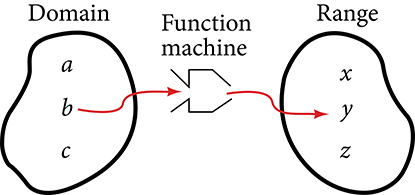
\includegraphics[height=35mm, width=80mm]{Chapter 3/3.2-figure1.jpeg}}

\vspace{3mm}

Visually, we can think of a function as a machine. The domain of a function is a holding area of input values. These input values can be thought of as raw or unprocessed material. 
\vspace{2mm}

Depending on the function's formula or rule, some processing occurs. For example, if the function is $$f(x)= 2x+3$$ the machine doubles the input and adds $3$. So if we put $x=4$ through the machine, this is how we are processing $4$:
$$ f(4)= 2(4) +3 $$
\vspace{2mm}

The output of the machine, or the final product is the value $f(x)$, which is determined by the processing. So the machine produces $f(4)=11$.
\vspace{2mm}

Since a function has many values in its domain and range, we want to handle these values using interval notation. 
\vspace{2mm}

Let's gets started...

    \newpage
 \begin{comment}
     \underline{\textbf{Example 2 - Finding the Domain of a Function as a Set of Ordered Pairs}}
   
    Find the domain and range of the following function: $$\{ (2,10), (3,10), (4,20), (5,30), (6,40)\}$$
    \vspace{5mm}
    Domain: 
   
    Range: 
 \end{comment}  

\begin{boxR}
    \textbf{How To}
    \vspace{1mm}
    \hline
    \vspace{2mm}
    \textbf{Given a function written in equation form, find the domain.}
    \begin{enumerate}
        \item Identify the input values.
        \item Identify any restrictions on the input.
        \item Write the domain in interval notation if possible, considering the input values with the restrictions in consideration.
    \end{enumerate}
\end{boxR}
\vspace{1mm}

\underline{\textbf{Example 2 - Identifying Tables that Represent Functions}}

Find the domain of the function $f(x)=x^2-1$ in interval form.

\vspace{35mm}

\begin{boxR}
    \textbf{How To}
    \vspace{1mm}
    \hline
    \vspace{2mm}
    \textbf{Given a function written in equation form that includes a fraction, find the domain.}
    \begin{enumerate}
        \item Identify the input values.
        \item Identify any restrictions on the input. Set the denominator equal to zero and solve for $x$.
        \item Write the domain in interval notation if possible, considering the input values with the restrictions in consideration.
    \end{enumerate}
\end{boxR}
\vspace{1mm}


\underline{\textbf{Example 3 - Find the Domain of a Function Involving a Denominator}}
\vspace{1mm}

Find the domain for the function $\D f(x) = \frac{x+1}{2-x}$ in interval notation. 
    \newpage


\begin{boxR}
    \textbf{How To}
    \vspace{1mm}
    \hline
    \vspace{2mm}
    \textbf{Given a function written in equation form including an even root, find the domain.}
    \begin{enumerate}
        \item Identify the input values.
        \item Identify any restrictions on the input: since there is an even root, exclude any real numbers that result in a negative number in the radicand. Set the radicand greater than or equal to zero and solve for $x$.
        \item The solution(s) from step 2 are the domain of the function. Write answer in interval form.
    \end{enumerate}
\end{boxR}
\vspace{1mm}
 
\underline{\textbf{Example 4 - Find the Domain of a Function With an Even Root}}

Find the domain of the function $f(x)=\sqrt{7-x}$.



\newpage

{\large \textbf{Finding the Domain and Range from Graphs}}

Another way to identify the domain and range of functions is by using graphs. Because the domain refers to the set of possible input values, the domain of a graph consists of all the input values shown on the $x$-axis. The range is the set of possible output values, which are shown on the $y$-axis. \emph{Keep in mind that if the graph continues beyond the portion of the graph we can see, the domain and range may be greater than the visible values.}

\vspace{3mm}

\underline{\textbf{Example 6 - Finding Domain and Range from a Graph}}

Find the domain and range of $f$ whose graph is shown below. 

\centerline {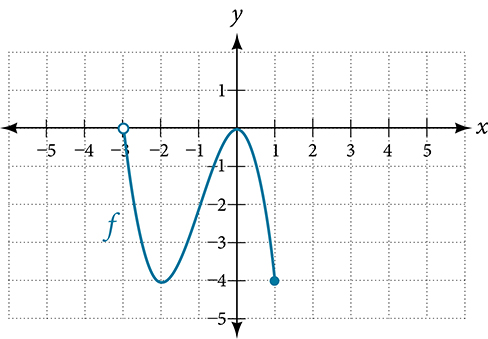
\includegraphics[scale=1.5]{Chapter 3/3.2-figure2.jpeg}}


\newpage

\underline{\textbf{Example 7 - Find the Domain and Range from a Graph of Oil Production}}

Find the domain and range of $f$ whose graph is shown below. 
\\

\centerline{ 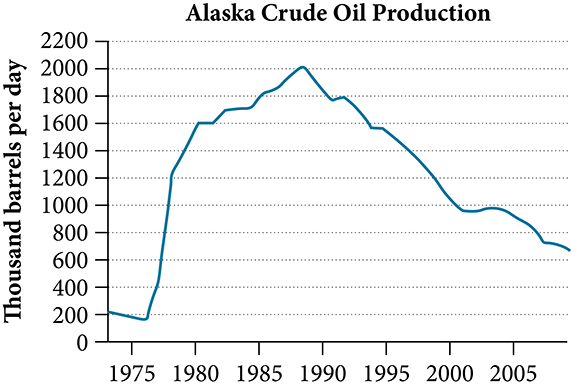
\includegraphics[scale=1.6]{Chapter 3/3.2-figure3.jpeg }}
\newpage

{\large \textbf{Graphing Piecewise-Defined Functions}}

Sometimes, we come across a function that requires more than one formula in order to obtain the given output. For example, we have worked with the absolute value function $f(x)= |x|$. 

If we input $0$, or a positive value, the output is the same as the input: 

$$ f(x) = x \text{ if } x \geq 0$$

If we input a negative value, the output is the opposite sign of the input (or we multiplied by $-1$):

$$ f(x) = x \text{ if } x < 0$$


Because $f(x)$  is defined differently depending on its input, the absolute value function is an example of a piecewise function.
\\

\begin{boxR}
    \textbf{Piecewise Function}
    \vspace{1mm}
    \hline
    \vspace{2mm}
    
A \textbf{piecewise function} is a function in which more than one formula is used to define the output. Each formula has its own domain, and the domain of the function is the union of all these smaller domains. We notate this idea as follows:

$$f(x) = \begin{cases} 
   \text{formula 1}, & \text{ if } x \text{ is in domain } 1 \\ 
    \text{formula 2}, & \text{ if } x \text{ is in domain } 2 \\ 
    \text{formula 3}, & \text{ if } x \text{ is in domain } 3 \\ 
    \end{cases} $$
\end{boxR}


In piecewise notation, the absolute value function is given as: 

\newpage

\underline{\textbf{Example 12 - Working with a Piecewise Function}}

A cell phone company uses the function below to determine the cost, $C$, in dollars for the gigabytes $g$ of a data transfer. 

$$ C(g) =  \begin{cases} 
   25 & \text{ if }  0 < g < 2 \\ 
   25+ 10(g-2) & \text{ if } g \geq 2 \\ 
    \end{cases} $$

Find the cost of using $1.5$ gigabytes of data and $4$ gigabytes of data. 

\vspace{70mm}

Analysis: 

\centerline{ 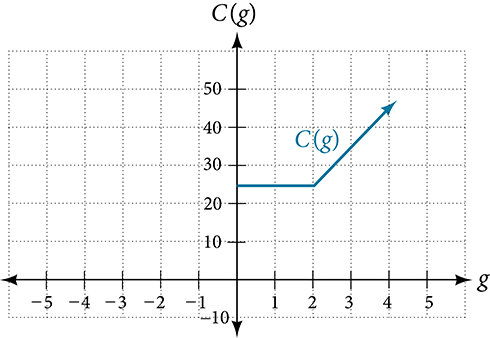
\includegraphics[scale=1.5]{Chapter 3/3.2-figure4.jpeg}}

\newpage
\underline{\textbf{Example 13 - Graphing a Piecewise Function}}

Sketch a graph of the function. 


$$ f(x) =  \begin{cases} 
   x^2 & \text{ if }  x \leq 1 \\ 
   3 & \text{ if } 1 < x \leq 2 \\ 
    x & \text{ if }  x > 2 \\ 
    \end{cases} $$



\newpage


\textbf{Toolkit Functions}
\\

 \begin{tabular}{ |c|c|c| } 
         \hline
              \textbf{Name} & \textbf{Function} & \textbf{Graph} \\
             \hline
             Constant & $f(x)=c$ where $c$ is a constant & 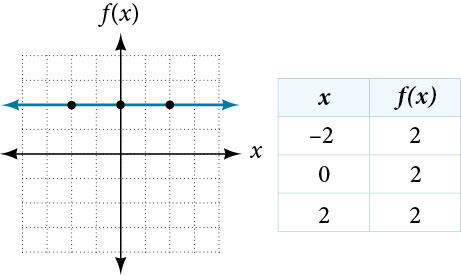
\includegraphics[]{Chapter 3/3.1-figure7.jpeg} \\
             \hline
            Identity & $f(x)=x$ & 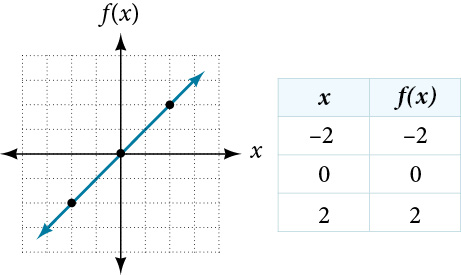
\includegraphics[]{Chapter 3/3.1-figure9.jpeg}\\
            \hline
            Absolute Value & $f(x)=|x|$ & 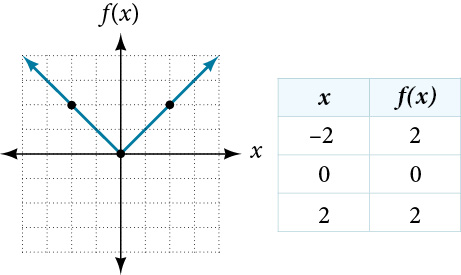
\includegraphics[]{Chapter 3/3.1-figure10.jpeg} \\
            \hline
             Quadratic & $f(x)=x^2$ & 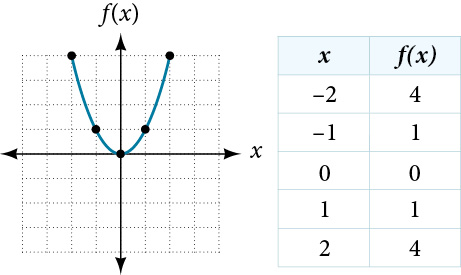
\includegraphics[]{Chapter 3/3.1-figure11.jpeg}\\
            \hline
          \end{tabular} 

\newpage

 \begin{tabular}{ |c|c|c|} 
         \hline
              \textbf{Name} & \textbf{Function} & \textbf{Graph} \\
            \hline
            Cubic & $f(x)=x^3$  &  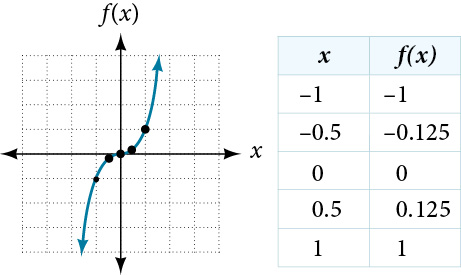
\includegraphics[scale=1]{Chapter 3/3.1-figure12.jpeg}\\
            \hline
            Reciprocal & $f(x) = \frac{1}{x}$ &  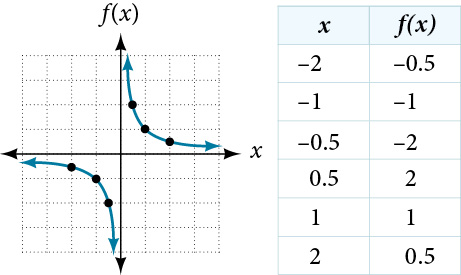
\includegraphics[]{Chapter 3/3.1-figure13.jpeg} \\
            \hline
            Reciprocal Squared & $f(x)=\frac{1}{x^2}$ & 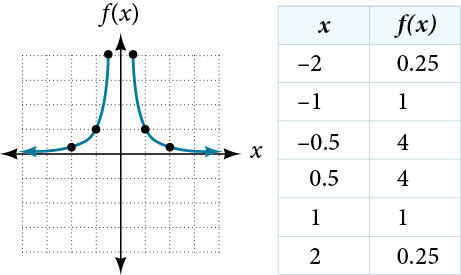
\includegraphics[]{Chapter 3/3.1-figure14.jpeg}\\
            \hline
            Square Root & $f(x)=\sqrt{x}$ & 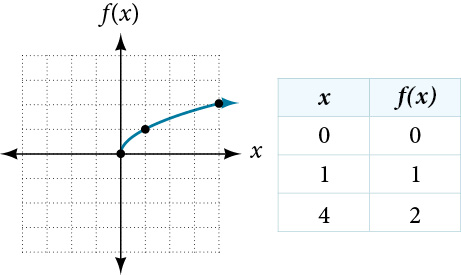
\includegraphics[]{Chapter 3/3.1-figure15.jpeg}\\
            \hline
            Cube Root & $f(x)=\sqrt[3]{x}$ & 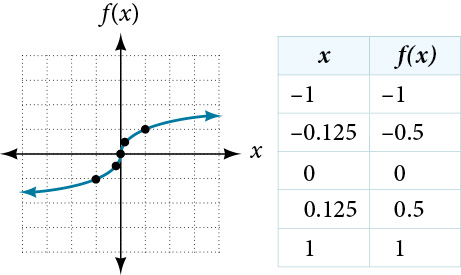
\includegraphics[]{Chapter 3/3.1-figure16.jpeg}\\
            \hline
             \end{tabular}










\end{document}


